% !TEX program = xelatex
\documentclass[11pt,a4paper]{article}
\usepackage[margin=1in]{geometry}
\usepackage{graphicx}
\usepackage{longtable}
\usepackage{hyperref}
\usepackage{booktabs}
\usepackage{enumitem}
\usepackage{titlesec}
\usepackage{lscape}

% Section title formatting
\titleformat{\section}{\bfseries\Large}{\thesection}{1em}{}
\titleformat{\subsection}{\bfseries\large}{\thesubsection}{1em}{}

\hypersetup{colorlinks=true, linkcolor=blue}

\begin{document}

%=== Title Page ===
\begin{center}
  {\LARGE \bfseries Emotion‐Aware, Agentic Healthcare Chatbot Proposal} \\
  \vspace{0.5em}
  {Prepared by: Team QuantumWar}
\end{center}

\vspace{1em}

%=== Problem Statement ===
\section{Problem Statement}
Modern Chatbot health interactions lack two critical capabilities:
\begin{enumerate}[left=0pt,label=\arabic*)]
  \item \textbf{Emotional Intelligence:} Traditional chatbots “hear” what patients say but ignore how they say it – anxiety and distress go unnoticed.
  \item \textbf{Modular Expertise \& Memory:} Monolithic dialogue models struggle with medical accuracy and conversational empathy, and lack persistent memory across sessions.
\end{enumerate}

\textbf{Goal:} Build a real‐time, multi‐agent healthcare chatbot that:
\begin{itemize}[left=0pt]
  \item Detects and adapts to patient emotion in real time.
  \item Maintains a multimodal memory of content and affective state.
  \item Extracts symptoms, performs RAG‐powered medical lookups, suggests diagnoses.
  \item Recommends and books appointments with nearby doctors based on location and specialty.
\end{itemize}

%=== Solution Overview ===
\section{Solution Overview}
Our design leverages \textbf{LangGraph} orchestration, specialized LLM agents, speech modules (VAD, STT, TTS), and a high‐performance vector memory store:
\begin{enumerate}[left=0pt]
  \item \textbf{Emotion Detection Agent}: Analyzes pitch, tone, and pauses via VAD/STT i.e tags valence/arousal.
  \item \textbf{Multimodal Memory Agent}: Streams transcripts and emotion metadata into a vector DB (e.g., FAISS/Pinecone).
  \item \textbf{Specialized LLM Agents}: Symptom extraction, medical retrieval (RAG), empathy response, orchestrator.
  \item \textbf{Orchestration Layer}: LangGraph handles task decomposition, parallel execution, error handling.
  \item \textbf{Output \& Action}: Presents top‐3 differential diagnoses and enables appointment booking via scheduling APIs.
\end{enumerate}

%=== Technology Stack ===
\section{Technology Stack}
Below is a detailed technical stack mapping for each node/agent in the architecture, including their input/output (I/O) and implementation technologies.

\begin{longtable}{@{}p{0.22\textwidth}p{0.18\textwidth}p{0.18\textwidth}p{0.38\textwidth}@{}}
\toprule
\textbf{Agent/Node} & \textbf{Input} & \textbf{Output} & \textbf{Tech Stack / Tools} \\
\midrule
\endhead

Main Agent (Orchestrator) & User audio/text, context & Routed tasks to agents & LangGraph, Python, FastAPI \\
VAD & Raw audio & Speech segments & WebRTC VAD, PyAudio/SoundDevice \\
STT & Speech segments & Text transcript & OpenAI Whisper, Google STT, AssemblyAI \\
Emotion Detection & Transcript, audio features & Emotion tags & OpenSMILE, PyAudioAnalysis, Transformers \\
Memory Agent & Transcript, emotion tags & Embeddings in Vector DB & FAISS/Pinecone/Chroma, PostgreSQL/MongoDB, LangChain Memory \\
Empathy Response Agent & Utterance, emotion, context & Empathetic response & GPT‐4/Claude, LangChain, prompt engineering \\
Symptom Extraction & Text utterance & Structured symptom list & Bio\_ClinicalBERT, Med7, scispaCy, LangChain \\
Medical Retrieval (RAG) & Symptoms, context & Medical knowledge snippets & LangChain RAG, FAISS/Elasticsearch, Ollama \\
Task Breakdown & Complex intent & Sub‐task list & LangGraph, Python \\
Context Sharing & Sub‐agent outputs & Unified session context & LangGraph, Redis \\
Diagnosis Agent & Unified context & Top‐N diagnoses, doctor suggestions & GPT‐4/Claude, custom LLM function‐calls, hospital APIs \\
Doctor’s Dataset & Query params & List of doctors, booking links & PostgreSQL/MongoDB, RESTful APIs \\
Frontend & User input & Chat UI, emotion meter & React.js, WebSockets, Native SDKs \\
Monitoring & System logs/events & Metrics, alerts & Prometheus, Grafana, ELK Stack \\
\bottomrule
\end{longtable}

%=== System Architecture ===
\section{System Architecture}
\begin{landscape}
  \begin{figure}[h!]
    \centering
    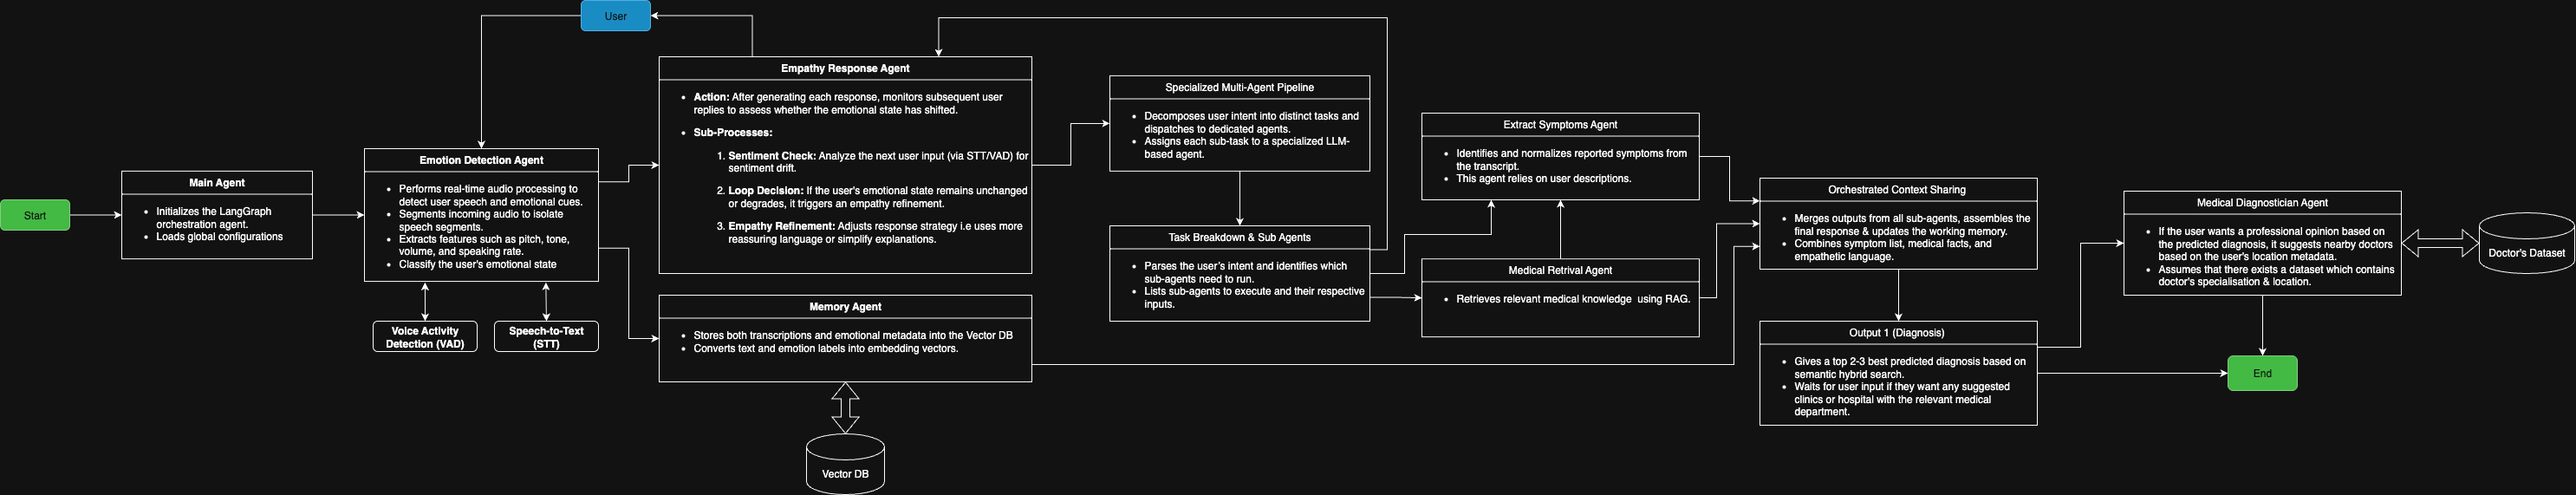
\includegraphics[height=0.32\textheight]{ChatBot_Healthcare_flow.png}
    \caption{Agentic Chatbot System Architecture}
    \label{fig:architecture}
  \end{figure}
\end{landscape}

\subsection{High‐Level Flow}
\begin{enumerate}[left=0pt]
  \item User speaks or types input (audio/text).
  \item VAD $\to$ STT $\to$ Emotion Detection Agent (real‐time paralinguistic analysis).
  \item Memory Agent ingests transcript + emotion tags into vector DB.
  \item LangGraph orchestrator decomposes intent, dispatches sub‐agents in parallel.
  \item Symptoms Extraction $\to$ Medical Retrieval (RAG lookup).
  \item Empathy Response Agent generates tone‐adaptive reply with sentiment loop.
  \item Diagnosis presentation + doctor recommendation + booking in conversation.
  \item Feedback loop: Next input monitored for sentiment drift; memory updated.
\end{enumerate}

\subsection{Key Modules}
\begin{longtable}{@{}p{0.25\textwidth}p{0.70\textwidth}@{}}
\toprule
\textbf{Module} & \textbf{Responsibility} \\
\midrule
STT \& VAD & Convert speech to text; detect voice activity, pitch, tone, and pauses. \\
Emotion Detection Agent & Classify valence/arousal; trigger empathy refinement if distress persists. \\
Memory Agent & Store multimodal embeddings in vector DB; support retrieval‐augmented prompts. \\
LangGraph Orchestrator & Define agent graph; handle task decomposition, parallelism, context sharing, and fallbacks. \\
Symptoms Extraction Agent & Normalize free‐form input into structured symptom lists. \\
Medical Retrieval Agent & Query curated clinical guidelines and disease ontologies via RAG. \\
Empathy Response Agent & Generate responses modulated by real‐time emotion checks. \\
Appointment Booking & Suggest specialists (geolocation + doctor dataset); integrate scheduling APIs. \\
\bottomrule
\end{longtable}

%=== Core Features & UX ===
\section{Core Features \& User Experience}
\begin{itemize}[left=0pt]
  \item \textbf{Emotion‐Adaptive UX}: Live emotion meter; adapt dialogues between clinical and empathetic tones.
  \item \textbf{Persistent Multimodal Memory}: Recall past diagnoses, medications, and emotional context across sessions.
  \item \textbf{Symptom‐to‐Diagnosis Pipeline}: NL symptom extraction $\to$ RAG lookup $\to$ ranked differential diagnoses with confidence.
  \item \textbf{Conversational Booking}: From symptoms to confirmed appointment in three conversational turns.
\end{itemize}

\section{Prototype Development:}
\item Build a proof-of-concept prototype integrating automated speech-to-text, emotion detection, symptom extraction, RAG-based medical retrieval, and top‑3 diagnosis generation to validate feasibility, test critical integration points, and gather early performance metrics.
    \begin{itemize}[label=--]
      \item Automated speech-to-text conversion and emotion detection to capture user input.
      \item Symptom extraction and normalization via the Extract Symptoms Agent.
      \item Medical context retrieval using RAG in the Medical Retrieval Agent.
      \item Generation of the top‑3 candidate diagnoses in the Orchestrated Context Sharing module.
    \end{itemize}
    This end-to-end prototype will validate feasibility, assess integration points, and provide early performance metrics.
\end{itemize}

%=== Technology Stack Summary ===
\section{Technology Stack Summary}
\begin{tabular}{@{}ll@{}}
\toprule
\textbf{Layer} & \textbf{Technologies} \\
\midrule
Orchestration & LangGraph \\
LLM APIs & OpenAI GPT‐4, Anthropic Claude \\
Speech Modules & WebRTC VAD, Whisper STT, Amazon Polly / Azure TTS \\
Vector Memory & FAISS, Pinecone, Chroma \\
Backend & Python, FastAPI, Docker, Kubernetes \\
Databases & PostgreSQL, MongoDB, Redis \\
Frontend & React.js, Native SDKs \\
Monitoring & Prometheus, Grafana, ELK Stack \\
Scheduling APIs & Calendly, Hospital Scheduling System APIs \\
\bottomrule
\end{tabular}

%=== Scalability, Security & Privacy ===
\section{Scalability, Security \& Privacy}
\begin{itemize}[left=0pt]
  \item \textbf{Horizontal Scaling:} Containerized services, Kubernetes HPA for LangGraph and STT clusters.
  \item \textbf{Failover \& Redundancy:} Multi‐region LLM endpoints; fallback to on‐prem models (Ollama).
  \item \textbf{Data Privacy:} End‐to‐end encryption, HIPAA/GDPR compliance, user‐controlled memory purge.
  \item \textbf{Audit \& Logging:} Immutable logs, role‐based access controls, continuous security scans.
\end{itemize}

%=== Next Steps & Prototype Plan ===


%=== Conclusion ===
\section{Conclusion}
By combining multimodal emotion analysis, LangGraph agent orchestration, and RAG‐powered medical retrieval, our solution delivers an empathetic, accurate, and actionable healthcare chatbot. We anticipate significant improvements in patient engagement, satisfaction, and care efficiency.

\end{document}
